\section{Step 3: Live Gateway}\label{sec:live}

An offline score says how a model ranks flows extracted from a finished file. A gateway classifies flows that an exporter emits while packets are still arriving. Equal scores do not show that both pipelines see the same flows, so we check fidelity flow by flow. This step uses CIC-IoT2023 only.

\subsection{Testbed}\label{sec:testbed}

The testbed runs Mininet~2.3.0~\cite{lantz2010mininet} with Open vSwitch~\cite{pfaff2015ovs} under WSL2 Ubuntu~24.04 on a laptop (i5-8350U, no GPU). In the topology h1--s1--gw--s2--h2, h1 replays traffic with tcpreplay at $\times1.0$ timing, and the gateway gw captures on its s1-facing interface. The gateway runs NFStream~6.6.0 in live mode with the offline settings, a single meter and a 64\,MB capture buffer. Exported flows are classified in micro-batches (256 flows or 50\,ms) by the deployed tree; the gateway can install OVS drop rules for both directions of a host pair (Section~\ref{sec:response}).

\emph{Windows and harness.} For each capture we cut one 60\,s window that starts 1\,s after the last training flow started, so all replayed traffic comes from the test period. Boundary-spanning connections are removed on both the offline and the live side; the offline reference is NFStream run on the same window file. After each window the harness waits 30\,s, then until the gateway's counters are quiet for 5\,s, and clears OVS blocks, per-pair verdict counts and ARP state, because the windows come from different capture sessions that reuse addresses. The first no-limit run (run~1) and the one-core run used an earlier harness without the quiet wait and the reset. A cgroup quota (\texttt{systemd-run}) sets the gateway's CPU budget: no limit, one core or half a core.

\emph{Achieved replay rates.} tcpreplay could not reach the original rate of the heaviest windows: the DDoS-SYN window (388,686 packets in 22.31\,s, about 17,423 packets/s) was replayed at 9,045--13,434 packets/s, and the Mirai window (about 4,782 packets/s) at 2,664--3,685 packets/s, i.e.\ 52--77\% of the original rates. All live results hold at these rates only.

\subsection{Fidelity Check}\label{sec:fidelity}

\emph{Flow-by-flow match.} In run~1 (no CPU limit, ten windows) we matched live to offline flows by 5-tuple and order of appearance within the 5-tuple. Of 148,779 offline and 148,884 live flows, 148,756 match; 23 are offline-only and 128 live-only. Per window, 96.62--100\% of matched flows have identical packet and byte counts (the rest differ in flow-boundary timing), and 97.63--100\% receive the same verdict. Macro-F1 is 0.804 both offline and live (host-pair CIs [0.457, 0.823] and [0.456, 0.822]). Live extraction is thus near-identical to offline extraction, not identical. Live macro-F1 is computed on a different, smaller sample than the test set and is not comparable to the test-set score.

\emph{Packet accounting.} The packet ratio (packets in live over offline flows, per window) lies between 0.9919 and 1.0064, and NFStream reported zero kernel drops, including in the DDoS-SYN window at 12,271 packets/s (5.9\,Mbps) and the Mirai window at 3,685 packets/s (16.2\,Mbps).

\emph{Delay.} Inference is fast: median batch latency 0.44\,ms (median batch size 209). Latency comes from flow export: the median verdict arrives about 15\,s after a flow's last packet (the idle timeout), and the first verdict for an attacker pair 15--35\,s after its first packet. Detection is therefore per flow, not per packet.

\begin{table}[t]
\centering
\caption{Live runs, DDoS-SYN window (offline: 142,724 flows). Delay: median verdict after flow end. Macro-F1 over all windows of the run (half core: three windows). --: not recorded.}
\label{tab:repeats}
\footnotesize
\setlength{\tabcolsep}{3pt}
\begin{tabular}{lcccc}
\hline
Run & Replay (pps) & Live flows & Delay (s) & Macro-F1 \\
\hline
No limit 1 & 12,271 & 142,752 & 17.8 & 0.804 \\
No limit 2 & 11,611 & 160,242 & 30.9 & 0.804 \\
No limit 3 & 10,936 & 184,483 & 34.0 & 0.804 \\
One core   & 13,434 & -- & 21.5 & 0.810 \\
Half core 1 & 12,088 & 142,730 & 75.9 & 0.918 \\
Half core 2 & 11,831 & 160,475 & 97.0 & 0.917 \\
Half core 3 & 12,401 & 142,729 & 60.3 & 0.917 \\
\hline
\end{tabular}
\end{table}

\emph{Repeats and CPU budget.} We ran the no-limit and half-core settings three times each and the one-core setting once (Table~\ref{tab:repeats}). Live macro-F1 was stable (offline 0.914 on the half-core windows), with zero kernel drops and a DDoS-SYN packet ratio of 1.00 in every run. Flow construction varied with the achieved replay rate. At 12,088~packets/s or more, the live DDoS-SYN flow count matched offline within 0.02\%; at 11,611--11,831~packets/s it was 12\% higher, and at 10,936~packets/s 29\% higher, because slower replay stretches inter-packet gaps past the idle timeout and splits connections, while every packet is still captured. Equal macro-F1 despite flow counts that differ by up to 29\% shows again that equal scores do not imply equal flows. The CPU budget mattered only in the DDoS-SYN window (Fig.~\ref{fig:delay}). With one core, a backlog kept the CPU at about 100\% for 45--60\,s after the flood, into the BruteForce window (mean CPU 40.6\% there, against 0.8\% without a limit), although that window's median delay was 15.7\,s. With half a core the gateway fell behind and needed another 110--163\,s after the gap to clear its backlog, still without drops. CPU pressure thus caused lag, not loss, but the flood never filled the 64\,MB buffer. Peak memory was 980--1,025\,MB in every detection run, from NFStream's flow state and the Python runtime, not from the 222\,KiB tree.

\begin{figure}[t]
\centering
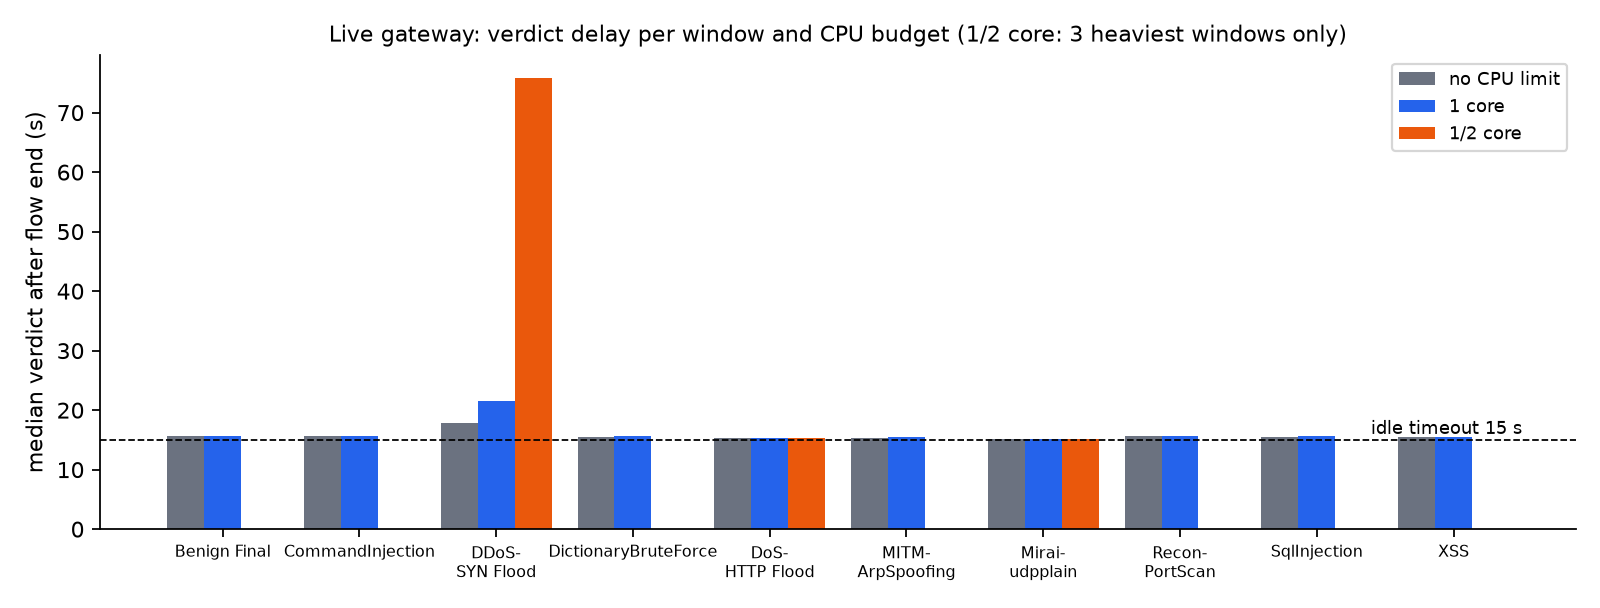
\includegraphics[width=\columnwidth]{../docs/figures/live_delay.png}
\caption{Median verdict delay after a flow's last packet, per window and CPU budget. Dashed: the 15\,s idle timeout. Half a core was tested on the three heaviest windows only.}
\label{fig:delay}
\end{figure}

\subsection{Failure Modes the Check Exposed}\label{sec:defect}

The fidelity numbers above hold only after three problems were fixed. None of them changed an offline score: at end of file every remaining flow is flushed, so features, labels and scores come out correct however late the flows would have been exported live.

\emph{A forwarding pitfall.} Replayed frames carry the source MACs of many capture devices. A MAC-learning switch maps all of them to h1's port and never forwards frames addressed to them, so part of the traffic silently never reaches the detector. Packet accounting reveals this; one OVS rule that forwards everything from h1 to gw fixes it.

\emph{Quiet meters.} NFStream checks a meter's timeouts only when that meter receives a packet, so idle flows can wait in a meter that receives none. We use one meter and run a 200\,packet/s background ping between h1 and h2 on a management subnet that is never scored or blocked.

\emph{An exporter defect.} With unmodified NFStream~6.6.0, verdicts came tens of seconds after the idle timeout. \texttt{NFCache}, an LRU \texttt{OrderedDict}, moves a key to the most-recently-used end only in \texttt{\_\_setitem\_\_}, but \texttt{consume()} updates an existing flow in place, so the cache stays in creation order. \texttt{meter\_scan()} expires flows from the head and stops at the first non-idle flow. One long-lived active flow, such as the background ping, therefore blocks the idle expiry of every flow behind it until its 120\,s active timeout. A one-line fix, \texttt{cache.move\_to\_end(flow\_key)} in the update branch, restores LRU order without changing flow boundaries or features. It cut the median delay after flow end from 82.5\,s to 15.6\,s (SQLi window) and from 49.2\,s to 15.5\,s (XSS). In the unpatched XSS run, only 64.5\% of the offline packets were in exported flows when the run stopped; on a continuously running gateway these flows would be exported late, not lost. A two-flow synthetic pcap reproduces the defect offline (export order A, B, A unpatched; B, A, A patched). Pekar and Jozsa map NFStream to CICFlowMeter features and leave the causes of value differences, such as ``how flows are updated and terminated'', out of scope~\cite{pekar2024integrity}; this defect is one such mechanism. To our knowledge its cause was previously undiagnosed. We reported it as nfstream\#262~\cite{nfstream262} and submitted the fix with a regression test as PR \#263~\cite{nfstream263}.\footnote{The symptom was reported without a cause in nfstream \#120~\cite{nfstream120} (2022) and \#193. It differs from \#196, \#215 and PR \#227, where the exporter's timer does not advance while no packets arrive; the background ping works around that problem, not around the ordering defect.}
